\section{Introduzione}
    La memoria è un componente fondamentale di un sistema di calcolo. Possiamo immaginarla come un grande vettore di byte, da cui un processo legge le istruzioni sulla base del program counter, e su cui può eseguire ulteriori operazioni di lettura e scrittura.
    
    \subsection{Hardware di base}
        La memoria centrale e gli indirizzi incorporati nel processore sono le uniche aree di memoria a cui la CPU può accedere direttamente. Pertanto, le istruzioni devono risiedere in una di queste due locazioni, e se così non è devono essere caricate prima di essere considerate disponibili.
        
        L'accesso alla memoria integrata del processore è estremamente rapido, e arriva a elaborare una o, in alcuni processori, più istruzioni per ciclo di clock. Tuttavia, accedere alla memoria centrale può richiedere molti cicli di clock e causa uno \textbf{stallo}, ossia una situazione in cui la CPU non dispone delle istruzioni per continuare. Ci avvaliamo quindi di una memoria veloce che si frappone fra memoria centrale e memoria interna del processore, comunemente chiamata \textbf{cache}, la quale si trova sul chip della CPU.
        
        Non è sufficiente garantire un accesso rapido alla memoria, in quanto l'accesso deve anche essere corretto; con ciò intendiamo che dobbiamo proteggere i processi di sistema dall'accesso di processi utenti, e, in sistemi multiutente, i processi utenti da processi di altri utenti. Questo tipo di protezione avviene solitamente, per motivi di efficienza, a livello hardware, e ci sono diversi modi per metterlo in atto.
        
        Innanzitutto, bisogna assicurarsi che ogni processo abbia un proprio spazio di indirizzamento ben definito: questo può essere realizzato tramite un \textbf{indirizzo base}, ossia il più piccolo indirizzo a cui quel processo può accedere, e un \textbf{indirizzo limite}, che rappresenta la dimensione massima di memoria assegnabile al processo. Si verifica che ogni istruzione sia compresa fra l'indirizzo minimo e quello massimo, e in caso contrario si lancia una eccezione (\textit{trap}) che passa il controllo al sistema operativo il quale, a sua volta, interpreta l'eccezione come un errore fatale. Questo impedisce ai processi utenti di accedere, intenzionalmente o meno, a aree di memoria e strutture dati riservate al sistema operativo o a altri utenti.
        
        Il sistema operativo ha un ruolo privilegiato in tutto ciò, e infatti può accedere indiscriminatamente a tutte le aree di memoria; e ciò gli permette di fornire molti servizi che richiedono la manipolazione di queste aree di memoria, come caricare processi nei loro spazi di indirizzamento, eseguire il \textit{dump} di un processo in caso di errore, fare context switch etc.
        
    \newpage
    \subsection{Associazione degli indirizzi}
        In genere un programma risiede su disco sotto forma di file binario eseguibile. Per essere eseguito va caricato in memoria e inserito nel contesto di un processo. Mentre è in esecuzione può accedere alle istruzioni e ai dati in memoria, mentre quando termina l'esecuzione dichiara disponibile il suo spazio di memoria.
        
        Generalmente gli indirizzi presenti nel programma sono simbolici (come una variabile \texttt{count}), che verranno tradotti in indirizzi rilocabili (per esempio \textit{"14kb dall'inizio di questo modulo"}) e infine in indirizzi assoluti (l'indirizzo unico 31415).
        
        L'associazione di istruzioni e dati a indirizzi di memoria si può effettuare in qualsiasi passo del seguente percorso:
        \begin{itemize}
            \item \textbf{Compilazione.} Se è già nota la locazione che il programma andrà ad occupare, si può già generare del codice assoluto. Se quella locazione dovesse cambiare, sarà chiaramente necessario ricompilare il codice.
            
            \item \textbf{Caricamento.} In caso non fosse disponibile la conoscenza di cui prima, verrà generato \textbf{codice rilocabile}, che assumerà valore assoluto in fase di caricamento. Nel caso in cui dovesse cambiare l'indirizzo iniziale, sarà necessario ricaricare il codice utente.
            
            \item \textbf{Esecuzione.} Se durante l'esecuzione il processo può essere spostato da un segmento di memoria all'altro, si deve ritardare ulteriormente l'associazione degli indirizzi. Ciò richiede hardware specializzato. La maggior parte dei sistemi operativi general-purpose moderni impiegano questo metodo.
        \end{itemize}
        
    \subsection{Spazi di indirizzi logici e fisici}
        Un indirizzo generato dalla CPU è comunemente chiamato \textbf{indirizzo logico}, mentre un indirizzo visto dall'unità di memoria, cioè caricato nel registro dell'indirizzo di memoria (\textit{memory address register}, MAR) è normalmente chiamato \textbf{indirizzo fisico}.
        
        L'associazione eseguita nelle fasi di compilazione e caricamento producono indirizzi fisici e logici identici, mentre nella fase di esecuzione gli indirizzi differiscono.
        
        Abbiamo lo \textbf{spazio degli indirizzi logici} e lo \textbf{spazio degli indirizzi fisici} che sono semplicemente l'insieme degli indirizzi generati da un programma e l'insieme degli indirizzi fisici associati.
        
        Un primo metodo molto rudimentale consiste semplicemente nel sommare agli indirizzi generati dal programma utente l'indirizzo di base, chiamato in questo caso \textbf{indirizzo di rilocazione}. In questo modo il programma utente non vede mai i veri indirizzi fisici, ma opera solo sulla base degli indirizzi virtuali del programma. In questo caso esistono due tipi di indirizzi: gli indirizzi logici, che vanno da 0 a \textit{max}, e gli indirizzi fisici, da $r + 0$ a $r +$ \textit{max}.
        
        Il programma utente crede di operare solo dalle locazioni 0 a \textit{max}. Il concetto di mappare uno \textit{spazio di indirizzi logici} su uno \textit{spazio di indirizzi fisici} è fondamentale per una corretta gestione della memoria.
        
    \subsection{Caricamento dinamico}
        In base a ciò che abbiamo visto fino ad ora, era necessario che il codice e i dati di un processo fossero presenti in memoria nella loro interezza per essere eseguiti. Questo limitava le dimensioni di un processo alle dimensioni della memoria.
        
        Si può ricorrere quindi al \textit{dynamic loading}. Con questo metodo carichiamo in memoria il programma principale e quando esso richiama una procedura controlliamo innanzitutto che essa sia caricata in memoria: se così non è si richiama il \textit{linking loader} rilocabile per caricare la procedura e aggiornare le tabelle degli indirizzi del programma, e solo poi si esegue la procedura.
        
        Questo metodo è vantaggioso quando abbiamo una grande quantità di codice che si occupa di casi poco comuni. Caricare procedure poco usate solo quando servono può drasticamente ridurre la memoria occupata, anche se le dimensioni totali di un programma sono elevate.
        
    \subsection{Linking dinamico e librerie condivise}
        Le \textit{dinamically linked libraries}, o \textbf{DLL}, sono librerie di sistema che vengono collegate ai programmi utente quando questi vengono eseguiti.
        
        Questo strumento permette di caricare librerie a tempo di esecuzione, anziché di compilazione. Se così non fosse, ogni eseguibile avrebbe al suo interno una copia di librerie di sistema, con tutte le loro dipendenze, e ciò creerebbe una ridondanza non indifferente.
        
        Un secondo vantaggio sta nel fatto che le DLL possono essere condivise fra più processi, nonostante una sola copia della DLL risieda in memoria centrale, e per questo sono conosciute anche come librerie condivise.
        
        Troviamo un altro vantaggio nell'aspetto amministrativo; aggiornare una DLL vuol dire potenzialmente aggiornare centinaia di programmi contemporaneamente. Un programma infatti contiene informazioni sulla versione della libreria usata, e basta aggiornare queste per passare alla nuova versione.
        
        Il supporto per il linking dinamico e per le librerie condivise richiede il \textbf{supporto del sistema operativo}. Infatti, se i processi sono protetti l'uno dall'altro, solo il sistema operativo può controllare se una routine è contenuta in una libreria esterna e regolare l'accesso di più processi alla stessa libreria.

\section{Allocazione contigua della memoria}
    La memoria centrale deve contenere sia il sistema operativo, sia i vari processi utenti: per questo è necessario assegnare le diverse parti della memoria centrale nel modo più efficiente possibile. Trattiamo qui un primo metodo di allocazione della memoria, l'allocazione contigua.
    
    Solitamente la memoria centrale è divisa in due partizioni, una per il sistema operativo e una per i processi utenti; è necessario trovare un modo efficiente per disporre in memoria questi ultimi e deciderne l'allocazione una volta caricati dallo scheduler. Con l'allocazione contigua posizioniamo l'inizio del nuovo processo esattamente dopo la fine del precedente.
    
    \subsection{Protezione della memoria}
        Vale la pena ragionare sul problema della protezione della memoria. Possiamo sfruttare un'idea vista in precedenza, e definendo un indirizzo di rilocazione e un indirizzo limite possiamo ottenere una buona politica di protezione della memoria in funzione di quanto visto precedentemente.
        
        In questo caso l'indirizzo di rilocazione può essere l'indirizzo minimo di un processo, e l'indirizzo limite può essere l'intervallo fra il minimo e il massimo. Controllando questi intervalli possiamo proteggere il sistema dai processi, e i processi da altri processi.
        
        Inoltre lo schema con registro di rilocazione permette al sistema operativo di cambiare dinamicamente le proprie dimensioni. Questo è molto utile per esempio quando un dispositivo non viene usato da molto tempo; in quel caso lasciarne in memoria il driver sarebbe uno spreco.
        
    \subsection{Allocazione della memoria}
        Parlando ora dell'effettivo metodo di allocazione: possiamo allocare diverse partizioni, di dimensioni variabili, ognuna adatta a contenere esattamente un processo.
        
        Inizialmente vediamo tutta la memoria come disponibile, e possiamo vederla come un \textbf{buco} (\textit{hole}). Come vedremo, questo metodo di allocazione porta ad avere nel lungo periodo una serie di buchi di diverse dimensioni. Questo avviene quando andiamo a deallocare dei processi. Il buco che essi lasciano può accomodare un processo più piccolo (lasciando la memoria in uno stato non contiguo) o, molto raramente, identico.
        
        Quando dobbiamo eseguire un processo e non c'è un buco di dimensioni sufficienti, possiamo come soluzione banale rifiutare il processo e fornire un adeguato messaggio di errore, o metterlo in una coda di attesa e verificare che lo spazio lasciato da buchi contigui sia sufficiente.
        
        I criteri più usati per scegliere un buco libero fra quelli disponibili nell'insieme sono i seguenti:
        \begin{itemize}
            \item \textbf{First-fit:} Si sceglie il \textit{primo} buco abbastanza grande.
            
            \item \textbf{Best-fit:} Si assegna il \textit{più piccolo} buco in grado di contenere il processo. A meno che non siano ordinati per dimensione, va eseguita una ricerca totale. Questo produce i buchi più piccoli dopo l'assegnazione.
            
            \item \textbf{Worst-fit:} Si sceglie il \textit{più grande} buco disponibile. Anche in questo caso va eseguita una ricerca totale a meno di un insieme ordinato. I buchi lasciati possono essere più utili dei precedenti in quanto è più probabile che accomodino processi futuri.
        \end{itemize}
        
        Tramite simulazioni si è dimostrato che first-fit e best-fit sono i migliori in termini di risparmio di tempo e utilizzo di memoria. Tuttavia nessuno dei due è definitivamente migliore dell'altro.
        
    \subsection{Frammentazione}
        Con i criteri best-fit e first-fit abbiamo un problema di \textbf{frammentazione esterna}; questo avviene quando la memoria totale disponibile potrebbe accomodare uno o più processi ma non è disposta in maniera contigua, e quindi risulta inutilizzabile. Statisticamente, per ogni \textit{n} blocchi di memoria, 0.5\textit{n} blocchi restano inutilizzati. Questa è nota come \textbf{regola del 50 per cento.}
        
        La frammentazione può essere \textbf{interna} oltre che esterna. Il concetto è simile alla frammentazione esterna ma avviene internamente alla partizione, e in particolare è lo spazio inutilizzato all'interno della partizione.
        
        Una soluzione alla frammentazione esterna può essere la \textbf{compattazione}. Consta semplicemente nel riordinare le porzioni di memoria allocata in maniera da formare un unico blocco e un unico buco. Questo tuttavia non è sempre possibile e anche quando lo è, può essere oneroso.
        
\section{Paginazione}
    Un'altra soluzione al problema della frammentazione potrebbe essere la \textbf{paginazione}, che permette di assegnare memoria ai processi ovunque essa sia disponibile. Essa evita inoltre problemi relativi alla frammentazione esterna e la necessità di compattazione. Dati i vari vantaggi che offre, è impiegata di frequente, da server di grandi dimensioni a dispositivi mobili.
    
    Per implementare ciò ci avvaliamo di una collaborazione fra hardware e software.
    
    \subsection{Metodo di base}
        Il metodo di base per implementare la paginazione consiste nel dividere la memoria fisica in blocchi di dimensione fissa detti \textbf{frame} e la memoria logica in blocchi di pari dimensione detti \textbf{pagine}.
        
        Abbiamo dunque due parti che compongono ogni indirizzo della CPU: un \textbf{numero di pagina}, che serve come indice per la tabella delle pagine, e un \textbf{offset di pagina}, che è la posizione all'interno del frame a cui viene fatto riferimento.
        
        Descriviamo ora i passaggi adottati dalla Memory Management Unit per tradurre un indirizzo logico generato dalla CPU in un indirizzo fisico:
        \begin{itemize}
            \item Usare il numero di pagina come indice nella tabella delle pagine.
            
            \item Estrarre il numero di frame corrispondente dalla tabella della pagine.
            
            \item Sostituire il numero di pagina con il numero di frame.
        \end{itemize}
        
        L'offset non cambia e pertanto non viene sostituito; insieme al numero di frame determinano l'indirizzo fisico.
        
        La dimensione di una pagina è solitamente una potenza di 2 compresa fra i 4KB e 1GB. Questa scelta semplifica di molto la traduzione degli indirizzi logici in corrispondenti indice e offset. Se la dimensione dello spazio degli indirizzi logici è $2^m$ e la dimensione di una pagina è di $2^n$ byte, allora gli $m - n$ bit più significativi di un indirizzo logico indicano il numero di pagina e gli $n$ bit meno significativi l'offset di pagina.
        
        Con questo metodo eliminiamo il problema della frammentazione esterna, ma non quello della frammentazione interna. Infatti Se un processo occupa una pagina più un singolo byte, dobbiamo assegnargli due intere pagine. È facile intuire che questo problema può essere arginato definendo pagine piccole. Tuttavia avere molte pagine piccole causa un overhead non indifferente e rallenta la trasmissione di dati.
        
        Quando abbiamo necessità di caricare un processo in memoria, andiamo a verificare che la sua dimensione espressa in pagine sia più piccola del numero di pagine disponibili, anziché eseguire il test sull'unità di memoria grezza.
        
        Un aspetto importante della paginazione è la netta differenza fra memoria vista dal programmatore e memoria fisica. Il programmatore vede la memoria occupata dal processo come contigua, e del resto ricordiamo che è normale sia così; un programma utente non deve sapere i dettagli della disposizione della memoria, in quanto deve operare solo e soltanto sulla porzione di memoria a esso assegnato; il sistema operativo, d'altro canto, conosce i frame occupati, da quali processi sono occupati, e altre informazioni su come i processi sono disposti in memoria. Anche questo è normale, in quanto il sistema operativo ha il compito, fra le altre cose, di gestire la paginazione e di riferirsi a indirizzi fisici oltre che logici.
        
    \subsection{Supporto hardware alla paginazione}
        Siccome ogni processo ha la sua tabella delle pagine, il puntatore alla stessa viene memorizzato nel PCB insieme ai valori di altri registri.
        
        La tabella delle pagine può essere implementata in molti modi diversi dal punto di vista hardware. Un modo molto semplice è implementarla come una serie di registri dedicati ad alta velocità. Questo rende la traduzione dell'indirizzo molto veloce ma aumenta i tempi dei cambi di contesto, in quanto ogni volta dovranno essere scambiati tutti i registri.
        
        La tabella degli indirizzi poò alternativamente essere mantenuta in memoria principale mentre un \textbf{registro di base della tabella delle pagine} (\textit{page-table base register}, PTBR) punta alla stessa. Così facendo il cambio di contesto ha tempi considerevolmente ridotti.
        
        \subsubsection{TLB}
            La tecnica appena descritta fa guadagnare tempo sui cambi di contesto ma rende l'accesso più lento. In questo caso infatti dobbiamo accedere alla memoria due volte, una per l'elemento della tabella delle pagine e una per il dato effettivo.
            
            La soluzione tipica a questo problema consiste nell'utilizzo di un \textbf{TLB} (\textit{translation look-aside buffer}), ossia uno speciale tipo di memoria. È infatti una memoria associativa; è una serie di coppie chiave-valore, ma riesce a confrontare un elemento che gli viene presentato contemporaneamente con tutte le chiavi, riportando dunque un valore molto velocemente.
            
            Tuttavia la TLB deve essere di dimensioni ridotte per una serie di motivi, fra cui il costo di una componente hardware così specializzata. Questo ci porta a capire l'utilizzo della TLB; essa contiene un piccolo numero degli elementi della tabella delle pagine, e quando la CPU genera un indirizzo logico si presenta il suo numero alla TLB. Se esso è presente, il numero del frame è immediatamente possibile per l'accesso, altrimenti si verifica un \textbf{insuccesso della TLB} (\textit{TLB miss}), e si deve consultare la tabella delle pagine in memoria. I numeri ottenuti vengono così usati per l'accesso e inseriti nella TLB, così da rendere più rapidi i prossimi accessi.
            
            Quando la TLB è piena va scelto un elemento da rimuovere, e questo può avvenire in base a varie politiche, dalla strutturata \textbf{LRU} (\textit{least recently used}) fino a una politica round-robin, e addirittura una scelta casuale. Questo varia da CPU a CPU e alcune di esse consentono ad alcuni elementi di essere \textit{wired down}, ossia di non poter essere rimossi dalla TLB; questo solitamente si fa con elementi per il codice base del kernel.
            
            La percentuale di volte che il numero di pagina interessato si trova nel TLB è detta \textit{hit ratio}, e può esserci utile per calcolare il tempo medio di accesso alla memoria, tramite una somma fra il tempo di accesso in caso di \textit{TLB hit} e quello in caso di \textit{TLB miss}, pesati in base alla probabilità che appena definita (\textit{hit ratio}).
            
    \subsection{Protezione}
        In un ambiente paginato, solitamente la protezione della memoria è assicurata dai bit di protezione associati a ogni frame, che determinano se da un pagina si può leggere e scrivere o se è disponibile solo in lettura. Siccome questi bit sono memorizzati nella tabella delle pagine e si deve passare da questa tabella a ogni accesso alla memoria, essi vengono sempre verificati e il tentativo di scrivere in una pagina di sola lettura causa un errore a livello hardware.
        
        Questo metodo si può facilmente perfezionare; possiamo fornire permessi di sola lettura, sola scrittura e sola esecuzione ed eventualmente combinarli fra loro.
        
        Associamo inoltre a ciascun elemento della tabella delle pagine un ulteriore bit, detto \textbf{bit di validità}, che verifica se la pagina richiesta è presente all'interno della tabella delle pagine e quindi se è un indirizzo accessibile dal processo. Quando ciò non si verifica viene generata un'eccezione ed è il sistema operativo a decidere se garantire l'accesso.
        
    \subsection{Pagine condivise}
        Un vantaggio della paginazione è la possibilità di condividere pagine e quindi codice. Immaginiamo per esempio una libreria standard come \texttt{libc} che è potenzialmente usata da tutti i processi: caricarla centinaia di volte in memoria sarebbe uno spreco.
        
        Se il codice è \textbf{rientrante} (ossia non auto-modificante, non cambia mai durante l'esecuzione), esso può essere condiviso. Questa natura di sola lettura del codice non deve essere lasciata alla sua intrinseca correttezza ma deve essere fatta rispettare dal sistema operativo.
        
        Oltre alle librerie, altre risorse frequentemente usate possono essere condivise, come sistemi di database, compilatori e interfacce.
        
\section{Struttura della tabella delle pagine}
    La tabella delle pagine può essere strutturata in diversi modi. Andiamo a descrivere due fra i più comuni.
    
    \subsection{Paginazione gerarchica}
        La maggior parte dei calcolatori moderni dispone di spazi di indirizzamenti molto grandi per i processi, e questo implica anche una grande tabella delle pagine, in un sistema a 32 bit fino a 4MB. Ovviamente allocare una tabella delle pagine di queste dimensioni per ogni processo, anche uno composto da poche istruzioni, è uno spreco. Una soluzione sarebbe dividere la tabella in parti più piccole.
        
        Un metodo per implementare ciò sarebbe indicizzare la tabella stessa in un'altra tabella esterna, e quindi dividere l'indirizzo logico come segue:
        
        \begin{figure}[h]
            \centering
            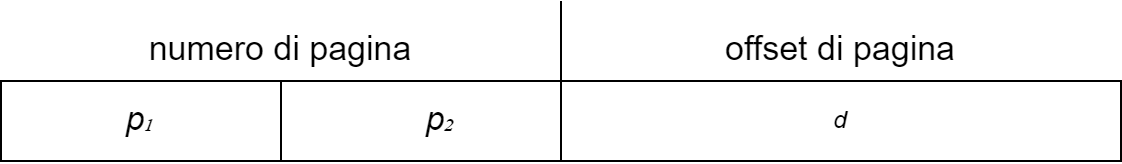
\includegraphics[width =0.8\textwidth]{img/paginazione.png}
            \caption{Divisione dell'indirizzo logico per la paginazione gerarchica}
            \label{fig:my_label}
        \end{figure}
        
        Questa soluzione non è più adatta nel caso di sistemi a 64 bit in quanto la tabella esterna sarebbe nuovamente troppo grande. La soluzione intuitiva è suddividere a tabella in più parti più piccole.
        
        Tuttavia nemmeno questo si dimostra fattibile, e in molti casi andrebbe ulteriormente aumentato il numero di livelli, arrivando in alcuni casi a sistemi di paginazione gerarchica a sette livelli- aumentando molto il numero di accessi alla memoria, e quindi diventando un modello poco desiderabile.
        
    \subsection{Tabella delle pagine invertita}
        Uno svantaggio dei metodi visti fino ad ora è che, dovendo la tabella delle pagine contenere tutti gli indirizzi virtuali di un processo, essa può arrivare a contenere anche milioni elementi, e quindi occupare una grande quantità di memoria fisica.
        
        Per risolvere questo problema si può fare uso della \textbf{tabella delle pagine invertita}. Una tale tabella ha un elemento per ogni pagina reale (o frame). Ciascun elemento è quindi costituito dall'indirizzo virtuale della pagina memorizzata in quel reale frame di memoria e informazioni relative al processo che possiede tale pagina.
        
        Abbiamo quindi una singola tabella per tutta la memoria, che ha un solo elemento per ogni pagina di memoria fisica. Sebbene questo metodo diminuisce lo spazio richiesto per la memorizzazione di tabelle (o in questo caso tabella) delle pagine, aumenta il tempo di ricerca di una pagina nella tabella, siccome la tabella invertita è ordinata per indirizzi fisici, ma i processi ragionano per indirizzi virtuali. Una tale richiesta renderebbe necessario esaminare tutta la tabella nel caso peggiore. Si può ridurre l'entità del problema introducendo una tabella hash, che introduce però un secondo accesso alla memoria (uno alla tabella hash, uno alla tabella della pagine).
        
        Un'altra questione interessante è relativa alla memoria condivisa: un singolo indirizzo non può essere condiviso da più processi impiegando una tabella delle pagine invertita.
        
\section{Swapping dei processi}
    Le istruzioni di un processo e i dati su cui operano devono essere in memoria centrale. Tuttavia un processo o una sua parte può essere temporaneamente rimosso dalla memoria (un'operazione detta \textit{swap out}), spostato in una memoria o partizione ausiliaria e susseguentemente essere ricaricato in memoria (\textit{swap in}). Questo procedimento, detto \textbf{swapping dei processi}, permette ai processi di indirizzare una quantità di indirizzi che eccedono l'effettiva dimensione della memoria fisica, aumentando così il grado di multiprogrammazione.
    
    \subsection{Swapping standard}
        Lo swapping standard è lo spostamento di interi processi fra la memoria centrale e un veloce dispositivo di archiviazione che deve essere abbastanza grande da contenere tutte le porzioni dei processi che devono essere memorizzati nonché fornire accesso diretto alle immagini dei processi memorizzati.
        
        Vanno conservate e quindi memorizzate nella memoria ausiliaria anche le strutture dati relative al processo ed eventualmente ai suoi thread e i metadati del processo, in quanto dovranno essere ripristinati.
        
        Una buona politica di swap out è muovere nella memoria ausiliaria i processi meno usati o comunque usati meno recentemente.